\documentclass{article} 
\usepackage{amsmath}
\usepackage{listings}
\usepackage{graphicx}
\begin{document}
\title{CS231n- Lecture 3}
\maketitle
\section{Optimization}
\ \subsection{Computational Graph}
We need to see computational graph. It's huge in Convolutional Neural Networks and Neural Turing Machine.\\
$f(x,y,z)=(x+y)z$ \\
e.g x=-2, y=5, z=-4\\
$q=x+y$ \\ $\frac{\partial q}{\partial x}=1$ \\ $\frac{\partial q}{\partial y}=1$
$f=qz$ \\ $\frac{\partial f}{\partial q}=z$ \\ $\frac{\partial f}{\partial z} = q$ \\
\\ We made a forward pass, now we'll make a backward one
$\frac{\partial f}{\partial f}=1$ \\
$\frac{\partial f}{\partial z}=x+y=3$ \\ The influence of z on f is three times in positive magnitude \\
$\frac{\partial f}{\partial q}=z=-4$ \\  if q increases by h, then f decreases by 4 times that magnitude
$\frac{\partial f}{\partial y} = \frac{\partial f}{\partial q} \frac{\partial q}{\partial y}=-4 * 1 = -4$ \\
Similarly, $\frac{\partial f}{\partial x} = -4$  \\
Example: $f(w,x)= \frac{1}{1+e^(-(w_0 x_0 + w_1 x_1 + w_2))}$
\begin{figure}
  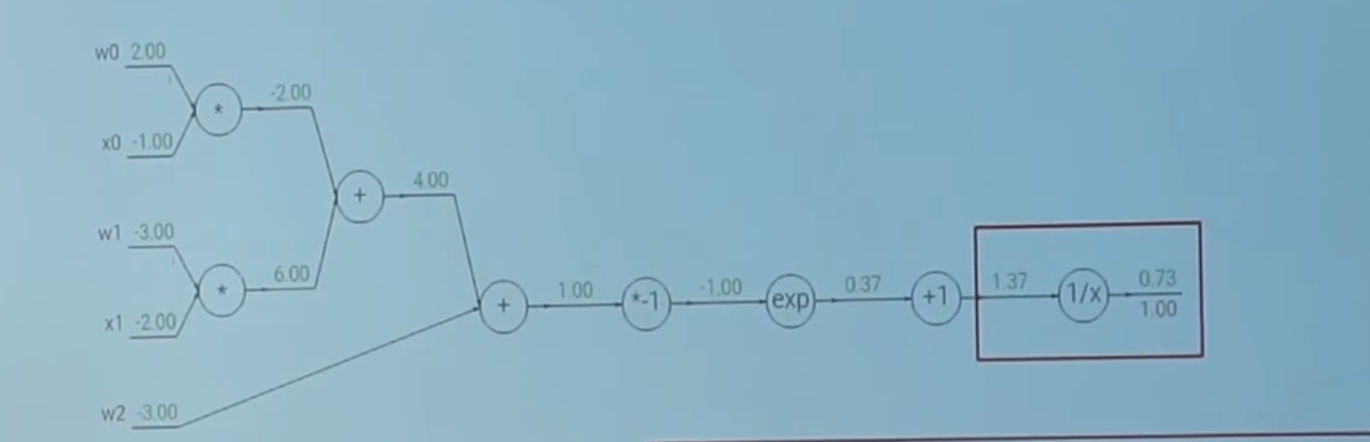
\includegraphics[width=\linewidth]{SS1.png}
  \caption{The Computational Graph}
  \label{fig:cGraph1}
\end{figure}
\\
\\
\\
\\ \\ \\ \\
\\
\\
\\
\\
$f(x) = e^x -> \frac{\partial f}{\partial x} = \frac{1}{x}$
\\$f(x) = \frac{1}{x} -> \frac{\partial f}{\partial x} = \frac{-1}{x^2}$
\\ So we get gradient at this position to be $\frac{-1}{1.37^2} * 1.00 = -0.53$
\\ Next level we get $1*(-0.53) = -0.53$
\\ This goes on and on, we multiply local gradient with the gates gradient
\begin{figure}
  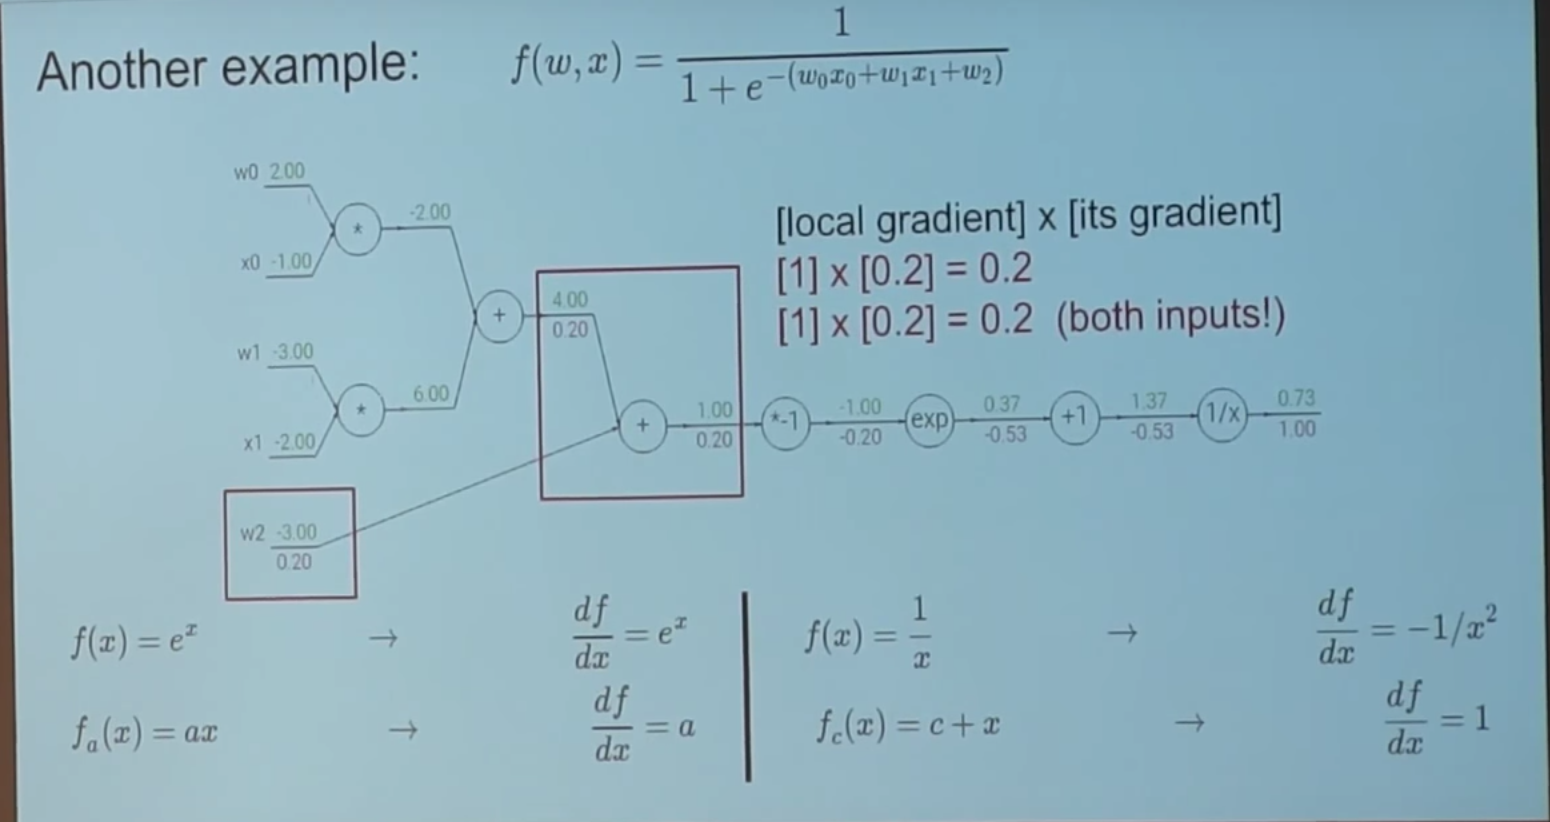
\includegraphics[width=\linewidth]{SS2.png}
  \caption{The Computational Graph after a few updates(AdditionGate)}
  \label{fig:cGraph1}
\end{figure}
\begin{figure}
  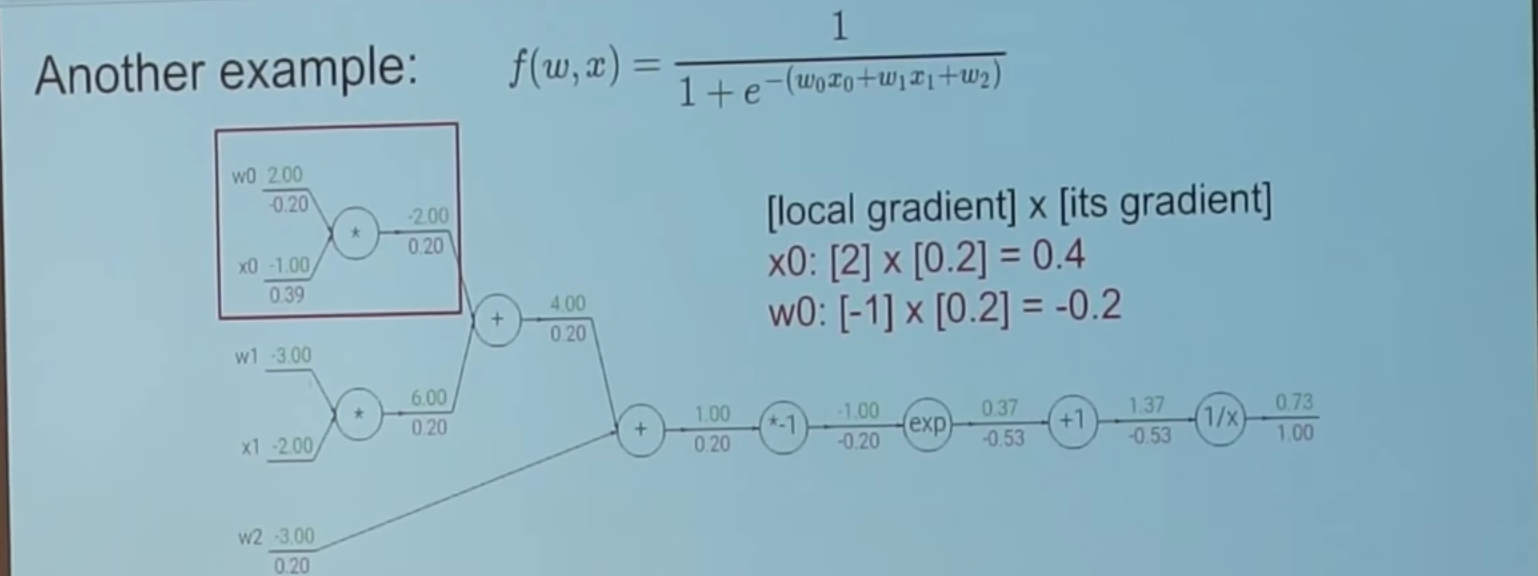
\includegraphics[width=\linewidth]{SS3.png}
  \caption{The Computational Graph after a few updates(MultGate)}
  \label{fig:cGraph1}
\end{figure}
\\
\\
\\
\\ \\ \\ \\
\\
\\
\\
\\
We can collapse into one sigmoid function
\\From now on rely on slides from "http://cs231n.stanford.edu/slides"
 only extra notes here.
\\ Understanding backward flow's intuition is very important.
\\ add gate is a gradient distributor. distributes equally
\\ max gate is a gradient router, larger one gets all the smaller gets 0. in backprop we are routing to the max value since only it contributes to the final thing. If equal, we just pick one but odds of it happening are rare.
\\ mul gate: gradient switcher
\\ there is never any loop in this. they are always DAGs
\\ Caching helps a lot sometimes
\\We need to do forward and backward for every gate. Forward computes loss, backwards analytical gradient and then updates. There is a separate CPU / GPu implement for each switch
\\ We generally use vectorized code where x,y,z are vectors. 
\\ We use Jacobian matrices to calculate a determinant
\\ Jacobian is a giant 4096 x 4096 matrix if we have 4096-d input vector and 4096-d output vectors
\\ Suppose $f(x)= max(0,x) (elementwise)$ then the Jacobian matrix with be a diagonal matrix.
\\ Jacobian in this case is a huge diagonal matrix with some 0s in it when x is neegative/0
\\ When we do minibatch with suppose 100 examples of the same we'll have 409600 * 409600 matrix so this is pretty huge
\\subsection{Neural Networks}
\\ Without the brain stuff
\\$X_{3072}  -W1-> h_{100} -W2-> s_{10}$ for CIFAR 10
\\ These 100-d vectors at $h_{100}$ can be seen as a hundred label thingy. Suppose we have 2 predict, cat and dog this can be seen as 100 different color cats and dogs which is again weighted.
\\ 3 Layer NN- $f= W_3 max(0, W_2 max(0, W_1 x))$
\\ syn - synapse
\\ Many types of Activation functions
\\ ReLU  , Leaky ReLU, Maxout etc. ReLU is generally used.
\end{document}
